% This is LLNCS.DEM the demonstration file of
% the LaTeX macro package from Springer-Verlag
% for Lecture Notes in Computer Science,
% version 2.4 for LaTeX2e as of 16. April 2010
%
\documentclass[english, 10pt]{llncs}
%
\usepackage{makeidx}  % allows for indexgeneration

\usepackage{epsfig}
\usepackage{multirow}
\usepackage[english]{babel}

%
\pagestyle{empty}

\newcommand{\tab}{\hspace{0.5cm}}

\begin{document}


%
\frontmatter          % for the preliminaries
%
%\pagestyle{headings}  % switches on printing of running heads
%\addtocmark{Model-Driven Engineering} % additional mark in the TOC
%
%
\title{Characterization of Adaptable Interpreted-DSML}

%
%\titlerunning{Characterization of Adaptable i-DSML}  % abbreviated title (for running head)
%                                     also used for the TOC unless
%                                     \toctitle is used
%
\author{Eric Cariou \and Olivier Le Goaer \and Franck Barbier \and Samson Pierre}
%
\authorrunning{Eric Cariou et al.} % abbreviated author list (for running head)
%
%%%% list of authors for the TOC (use if author list has to be modified)
\tocauthor{Eric Cariou, Olivier Le Goaer, Franck Barbier, and Samson Pierre}
%
\institute{Universit\'{e} de Pau / LIUPPA, PauWare Research Group, BP 1155,\\ F-64013 PAU CEDEX, France\\
\email{\{firstname.name\}@univ-pau.fr},
\texttt{http://www.pauware.com}
}

\maketitle 
             % typeset the title of the contribution
\thispagestyle{empty}

\begin{abstract}
 
One of the main goals of model-driven engineering (MDE) is the
manipulation of models as exclusive software artifacts. Model
execution is in particular a means to substitute models for code. More
precisely, as models of a dedicated domain-specific modeling language
(DSML) are interpreted through an execution engine, such a DSML is
called interpreted-DSML (i-DSML for short). On another way, MDE is a
promising discipline for building adaptable systems based on models at
runtime. When the model is directly executed, the system becomes the
model: This is the model that is adapted. In this paper, we propose a
characterization of adaptable i-DSML where a single model is executed
and directly adapted at runtime. If model execution only modifies the
dynamical elements of the model, we show that the adaptation can
modify each part of the model and that the execution and adaptation
semantics can be changed at runtime.

\keywords{model execution, adaptation, i-DSML, models at runtime}

\end{abstract}

\section{Problem of Interest}

As programming languages, domain-specific modeling languages (DSML) can be
compiled or interpreted. This distinction was early noticed by Mernik
\emph{et al.}~\cite{Mernik:2005} when comes the time to choose the most
suitable implementation approach for executable DSML:
\begin{itemize}
\item Compiled DSML: DSML constructs are translated to base language
  constructs and library calls. People are mostly talking about code
  generation when pointing at this approach;
\item Interpreted DSML: DSML constructs are recognized and interpreted
  using an operational semantics processed by an execution
  engine. With this approach, no transformation takes place, the model
  is directly executable.
\end{itemize}

With interpreted domain-specific modeling languages (the term i-DSML
is coined in \cite{clarke-book-iDSML13}), the ability to run a model
prior to its implementation is a time-saving and henceforth
cost-saving approach for at least two reasons: (a) It becomes possible
to detect and fix problems in the early stages of the software
development cycle and (b) ultimately the implementation stage may be
skipped. One slogan associated to i-DSML should be ``\textsl{what you
  model is what you get}'' (WYMIWYG). Meanwhile, software adaptation
and self-adaptive software~\cite{salehie09} have gained more and more
interest. Consequently, when building such software based on i-DSML,
the model has to be adaptable at runtime thus requiring to define
adaptable i-DSML.

\begin{figure}[htbp]
\begin{center}
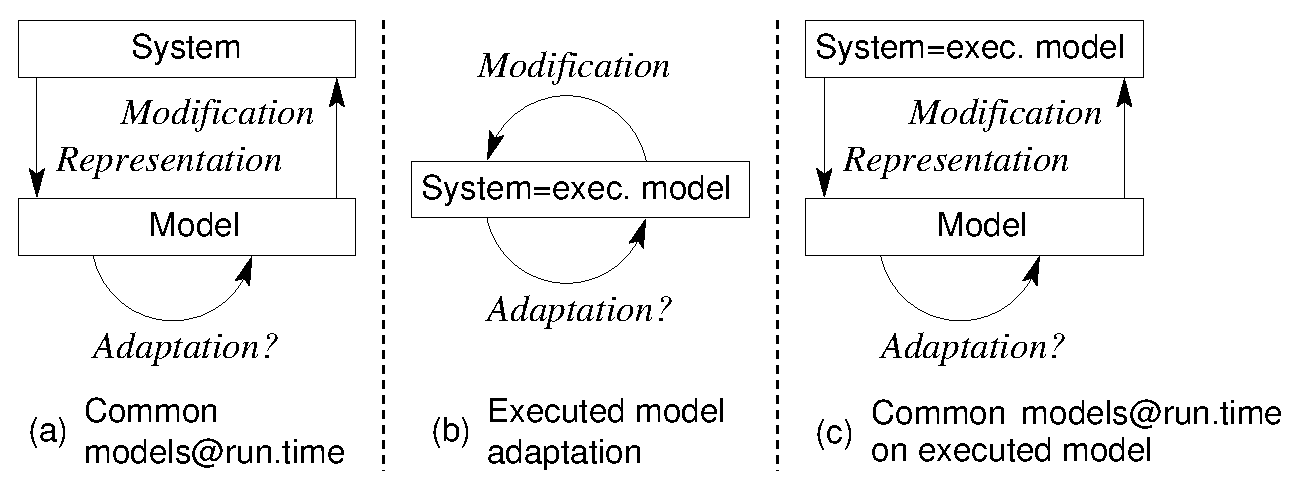
\epsfig{file=figures/loops2, width=9cm}
\caption{Adaptation loops}
\label{img_loops}
\end{center}
\end{figure}

The runtime adaptation problem is commonly tackled as a 2-stages
adaptation loop (analyze--modification). In the MDE (Model-Driven
Engineering) field, one of the most prominent way to implement this
loop is \textsl{models@run.time}~\cite{mart-computer09}, where models
are embedded within the system during its execution and acting
primarily as a reasoning support (case (a) in
figure~\ref{img_loops}). The main disadvantage of
\textsl{models@run.time} deals with maintaining a consistent and
causal connection between the system and the model for the model being
a valid representation of the system at runtime. The i-DSML approach
naturally circumvents this disadvantage since it suppresses the gap
between the system and the model: The system is the model being
executed. The reasoning is still made on the model but the required
modifications are then directly enacted on the model without needing a
representation of the system. Case (b) in figure~\ref{img_loops}
represents the adaptation loop in this new context. However, one major
requirement for adaptable i-DSML is that the executed model contains
all information necessary for both its execution and its
adaptation. This can sometimes lead to an increasing complexity of the
model and to a difficulty for managing the adaptation when mixing
together adaptation and execution. In this case, one can abstract all
the required information into a dedicated model for applying common
models@run.time techniques on a model execution system. This solution
is depicted by figure~\ref{img_loops}, case (c). The only difference
with the case (a) is simply that the system is of a special kind: A
model execution system. The problem of this solution is that it
reintroduces the causal link that we precisely try to avoid here. So,
both approaches (case (b) and (c)) are complementary and have pros and
cons. Depending on the context, one approach will be more suited than
the other one.

In this paper, we focus on the direct adaptation of an executed model
(case (b) of figure~\ref{img_loops}).
\cite{cariou-ciel12,cariou-mrt12} are first investigations on this
direct adaptation of executed models, that is, on adaptable i-DSML.
They establish what model execution adaptation is and how to express,
through a contract-based approach, that a model is consistent with an
execution environment (if not, the model has to be adapted). Based on
the same example of basic state machines and a train example, the
contribution of this paper consists in proposing a conceptual
characterization of adaptable i-DSML. The next section recalls what is
model execution and its well-known conceptual characterization. This
characterization is then extended in section~\ref{adaptable-iDSML} for
describing what an adaptable i-DSML contains and is based on. If model
execution only modifies the dynamical elements of the model, we show
that the adaptation can modify each part of the model and that the
execution and adaptation semantics can be changed at runtime. Finally,
related word is discussed before concluding.

\section{Characterization of i-DSML}
\label{iDSML-charaterization}

Defining executable models is not really a novel idea. Several papers
have already studied model execution, such
as~\cite{breton01,cariou-ecmfa11,clarke-book-iDSML13,combemale-jos09,combemale-apsec12,engels00,lehmann10,pons00}. All
these works establish a consensus about what the i-DSML approach
assumes:
\begin{itemize}
\item Executing the model makes sense. This is much more empirical
  evidence that shows us that some kinds of model are executable,
  others are not;
\item An engine is responsible for the execution of the model, that
  is, its evolution over time;
\item The model comes with all the information necessary for its
  execution through an engine: It is self-contained.
\end{itemize}

Before characterizing precisely what an i-DSML contains, we give a
better understanding of these three assumptions.

\subsection{Executable Nature of Models}

It exists a general classification of models that may help us to
identify models which have the ability to be executed or not: The
product--process duality. Indeed, models (and meta-models thereof) can
either express products or processes, regardless of the system
studied. By essence, only process models enable executability of their
content since they embody concepts closely related to the world of
runtime: Startpoint, endpoint, time (past/current/future), evolution
step, etc.
 
Applied to the field of software development standards, we can cite
SPEM as a process modeling language and CMW as a product modeling
language. As another OMG's prominent example, UML itself provides
three categories of diagrams, namely structure diagrams (Class,
Package, \dots), behavior diagrams (State Machines, Activity, \dots)
and interaction diagrams (Communication, Sequence, \dots). Logically,
only behavior and interaction diagrams may be executed. Beyond these
specific examples, when designing a DSML, it is important to keep in
mind its potential executable nature.

\subsection{Execution Engines}

An i-DSML is more than just a meta-model (abstract syntax and
well-formedness rules). A language definition also contains a concrete
syntax and semantics. The semantics of the language are captured in
the transformation rules in the case of compiled DSML or in the
execution engines in the case of interpreted DSML. An execution engine
is dedicated to a single i-DSML (UML state machines, SPEM, Petri nets,
etc.) and can execute any model conforming to this i-DSML.

The purpose of any execution engine is to ``play'' or to ``animate''
the model, making its state evolving, step by step. Execution
operations, implemented by the execution engine and potentially
attached to an element of the meta-model, manage each execution step
of the model. The current state of the model can be maintained locally
within the engine or, differently, embedded into the model itself. The
i-DSML approach singles out having self-contained models embedding
their current state but the former solution can be useful in some
cases. Typically, this is when one requires to execute models
conforming to a meta-model not designed for managing the current state
of the model, such as all the dynamic diagrams of UML. Indeed, the UML
standard does not define a current model state for any of these
diagrams that could be executable. In this case, the solution is to
store the current state of the model within the memory of the engine
or to extend the meta-model for managing a current model state. For
instance, \cite{cariou-ecmfa11} did it for UML state
machines. However, the extended meta-model differs from the UML
standard.

\subsection{Self-contained Executable Models}

When self-contained, the current state of the model being executed is
stored in the model itself. Thus, each execution step changes this
state. At first glance, this strategy seems to pollute the meta-model
with many details not relevant at design-time and seems to defeat the
abstraction offered by traditional modeling principles (a model is
the abstraction and a simplification of a given system). However,
there are two main reasons justifying to have self-contained models.

The first one is that it offers the major advantage that after each
execution step the current model state can be serialized into an
output file\footnote{That is why some authors may consider an
  execution process just as a sequence of endogenous model
  transformations, as explained in~\cite{cariou-ecmfa11}.}, thereby
providing a complete traceability of the execution as a sequence of
models. Some works, such as~\cite{breton01}, even
consider that the model can embed its complete execution trace in
addition to its current state. Based on this sequence of snapshots,
one can perform some useful operations like rollbacks, runtime
verification (such as the black-box execution verification
of~\cite{cariou-ecmfa11}), debugging, testing, and so forth.

The second and main reason is related to the essence of the executable
models. Such models aim at being substituted to the code, at the
lowest level, far away from abstract design models. Hence they have an
increased level of details and complexity required for their
executability. Moreover, executability being part of their nature, it
is unsurprising that they contain elements related to executability
such as the definition of their current state.

\subsection{The Design of an i-DSML}


\begin{figure}[htbp]
\begin{center}
\epsfig{file=figures/iDSL, width=12.5cm}
\caption{Conceptual framework for an i-DSML}
\label{iDSML}
\end{center}
\end{figure}


All elements required for model execution are located at the
meta-level. Indeed, a language is a self-contained i-DSML if one can
instantiate models that are executable through an execution
engine. One can identify a recurring pattern~\cite{combemale-apsec12}
about the constituents of an i-DSML (figure \ref{iDSML}):
\begin{enumerate}
	\item Meta-elements which express the organization of the process modeled,
	\item Meta-elements which express the state of the model being executed,
	\item Execution semantics which express how the model behaves when being executed.
\end{enumerate}

The item (1) is realized by traditional meta-modeling since the
engineers concentrate onto the static structure and associated
well-formedness rules of the models to be built. This is called the
Static Part. Item (2) introduces structural meta-elements intended to
store the state of the model at a given point of the time, also
associated with their well-formedness rules. This is called the
Dynamic Part. Last but not least, item (3) deals with defining how the
the model is evolving over time, modifying only the dynamic part
(\textit{i.e.} the static part never changes). An execution semantics
can be defined under several declinations. An axiomatic semantics
enables to complete the specification of the meta-model with
well-evolution rules defining the constraints on how the model
evolves~\cite{cariou-ecmfa11}. A translational semantics can be used
to apply simulation or verification techniques of another
technological space, such as in~\cite{combemale-jos09}. Finally, an
operational semantics is the operationalization of the execution
behavior in terms of actions through an action language and is
implemented by an execution engine. As depicted by the figure
\ref{iDSML}, the Dynamic Part and the Execution Semantics are specific
to i-DSML.


\subsection{Executable State Machines}

UML state machines are typically one of the best examples of
well-known executable models. In this paper, we then link our examples
to them but, for fluency, we define concise state machines restricted
to a limited number of features: Composite states with deep history
states and transitions associated with an event. Moreover, UML state
machines as defined by the OMG do not include a dynamic part as
required for a full-model execution (however \cite{cariou-ecmfa11}
proposes an extension of the UML meta-model for defining a dynamic
part for state machines).

\begin{figure}[htbp]
\begin{center}
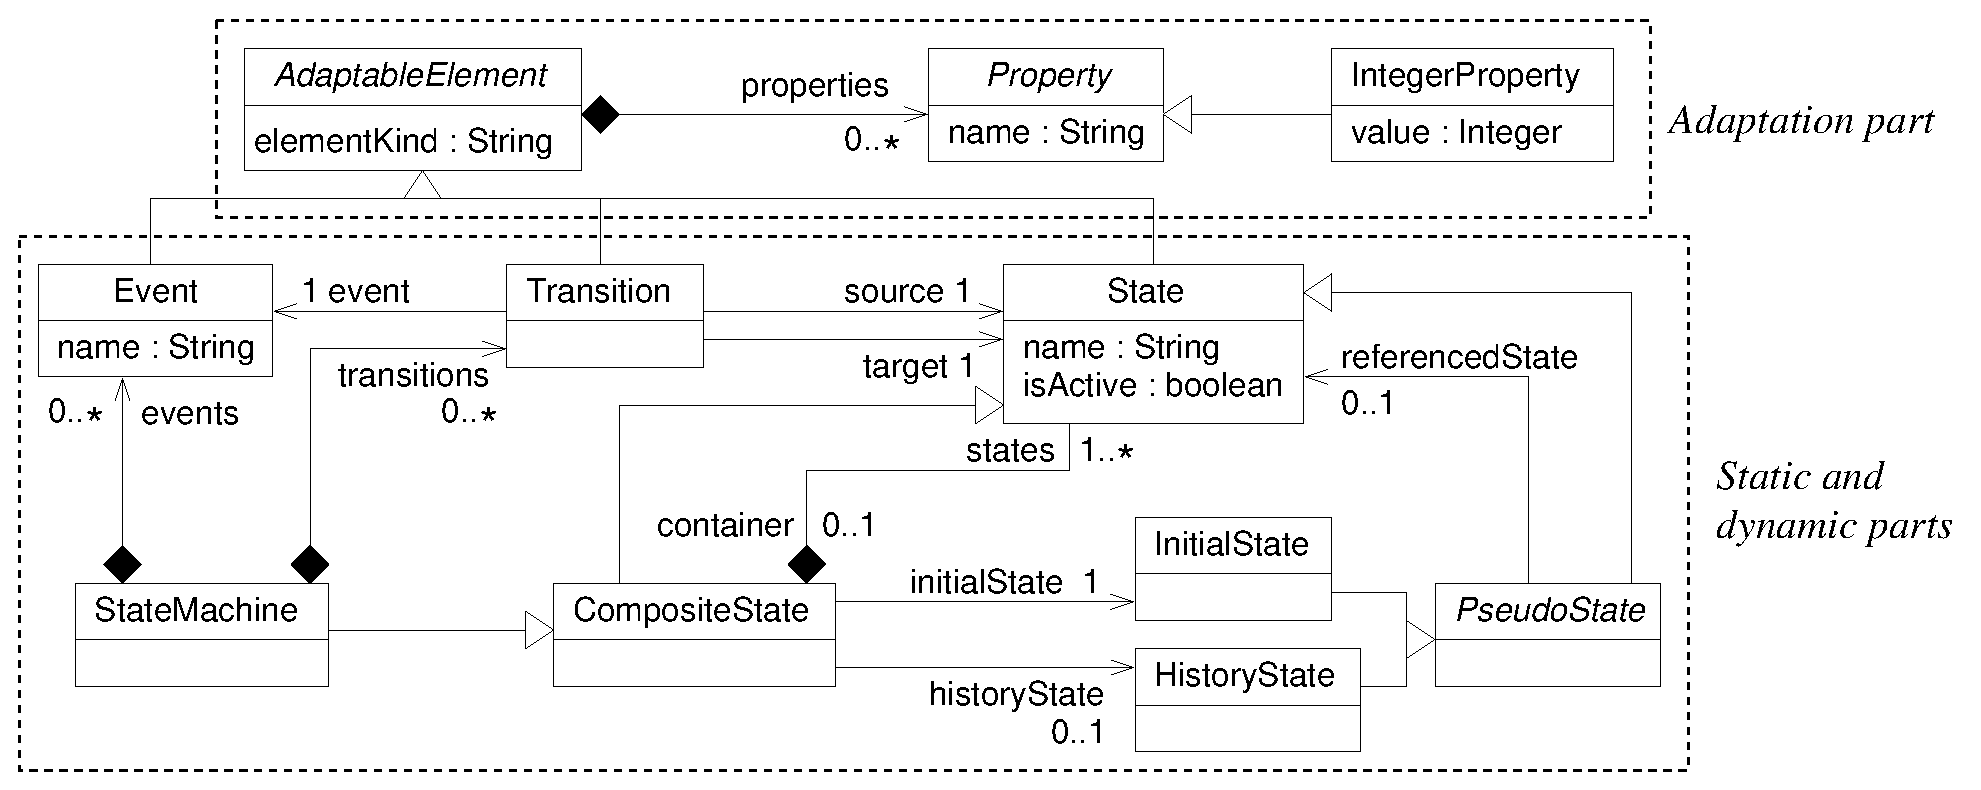
\epsfig{file=figures/mm-sm-adapt, width=12cm}
\caption{Meta-model of adaptable and executable basic state machines}
\label{mm-sm-adapt}
\end{center}
\end{figure}

The meta-model of our basic state machines is represented on
figure~\ref{mm-sm-adapt} (the \texttt{AdaptableElement} and
\texttt{[Integer]Property} elements are dedicated for managing the
adaptation and will be introduced in the next section). The static
part of the meta-model is composed of the following elements:
\begin{itemize}
\item A \textit{state} that is named and is contained in a
  \textit{composite state}.

\item Two kinds of \textit{pseudo states} can be defined: An
  \textit{initial state} and an \textit{history state}, each one
  referencing a state of the composite state to which they
  belong. Each composite state must have one and only one initial
  state. Having an history state (but only one) is optional.

\item A \textit{transition} between a source and a target states,
  associated with an \textit{event} that is simply defined with a
  name.

\item A \textit{state machine} is a special kind of composite
  state. It owns all transitions and events of the model and must be
  unique within the model.

\end{itemize}

The dynamic part of the meta-model is simply composed of two
elements. The first one is the \texttt{isActive} boolean attribute of
the \texttt{State} element. It enables to set that a state is
currently active or not. The second is the referenced state of an
history state that references the last active state of the composite
state to which it belongs. One can note that the
\texttt{referencedState} relation of a pseudo state is either playing
a static role (for an initial state) or a dynamic one (for an history
state). This state machine meta-model has been implemented in Ecore
for the EMF platform.

Static and dynamic parts are complemented with OCL invariants defining
the well-formedness rules for fully specifying the meta-model. For the
static part, it is for instance required to express that a pseudo
state references one of the states of its composite state. For the
dynamic part, the main invariant specifies the active state hierarchy
consistency: Either all the states are inactive (the model is not
being executed) or there is in the state machine one and only one
active state, and if this state is composite, it contains one and only
one active state and so on.

Concerning the execution semantics, both well-evolution rules, defined
using OCL, and an operational semantics, implemented by a
Kermeta\footnote{\texttt{http://www.kermeta.org/}} engine, have been
defined. For the sake of brevity, we will not present them. Just note
that their main goal is to define and to implement the main execution
step ensuring that, for an event occurrence, the right transition is
triggered depending on the current active states (that is, the active
state hierarchy is accordingly modified).

\subsection{A Train Example}

The example of this paper is freely inspired of a railway
system\footnote{The state machines of train behaviors and their
  associated signals of this paper are not at all intended to be
  considered as realistic specification of a railway system.}. The
behavior of a train is specified through a state machine. The train is
stopped or is running at a given speed, depending on the light signals along
the railway. The environment of execution of the train is the signals
that control its speed. Concretely, the different speeds of the
train are specified through the states of the state machine whereas
the signals are the events associated with the transitions between
these states. Within the same state machine, one can specify the
behavior of the system (the train) and its interaction with the
execution environment (the light signals).

\subsubsection{Execution Environment.}

The train is running on railways having signals with~3 or~4 different
color lights. There are two different kinds of railways: Normal speed
sections (up to 130 km/h) and high speed sections (up to 300
km/h). The signal with 3 colors is for normal speed sections while the
signal with 4 colors is for high speed ones. The meanings of the
colors are the following (only one light is put on at the same time):
\textit{red} means that the train must stop immediately,
\textit{amber} expresses that the train must not run at more that 40
km/h, \textit{green} means that the train can run at a normal speed
(but not more) and \textit{purple} that the train can run at a high
speed.

\subsubsection{Basic Train Model.}

\begin{figure}[htbp]
\begin{center}
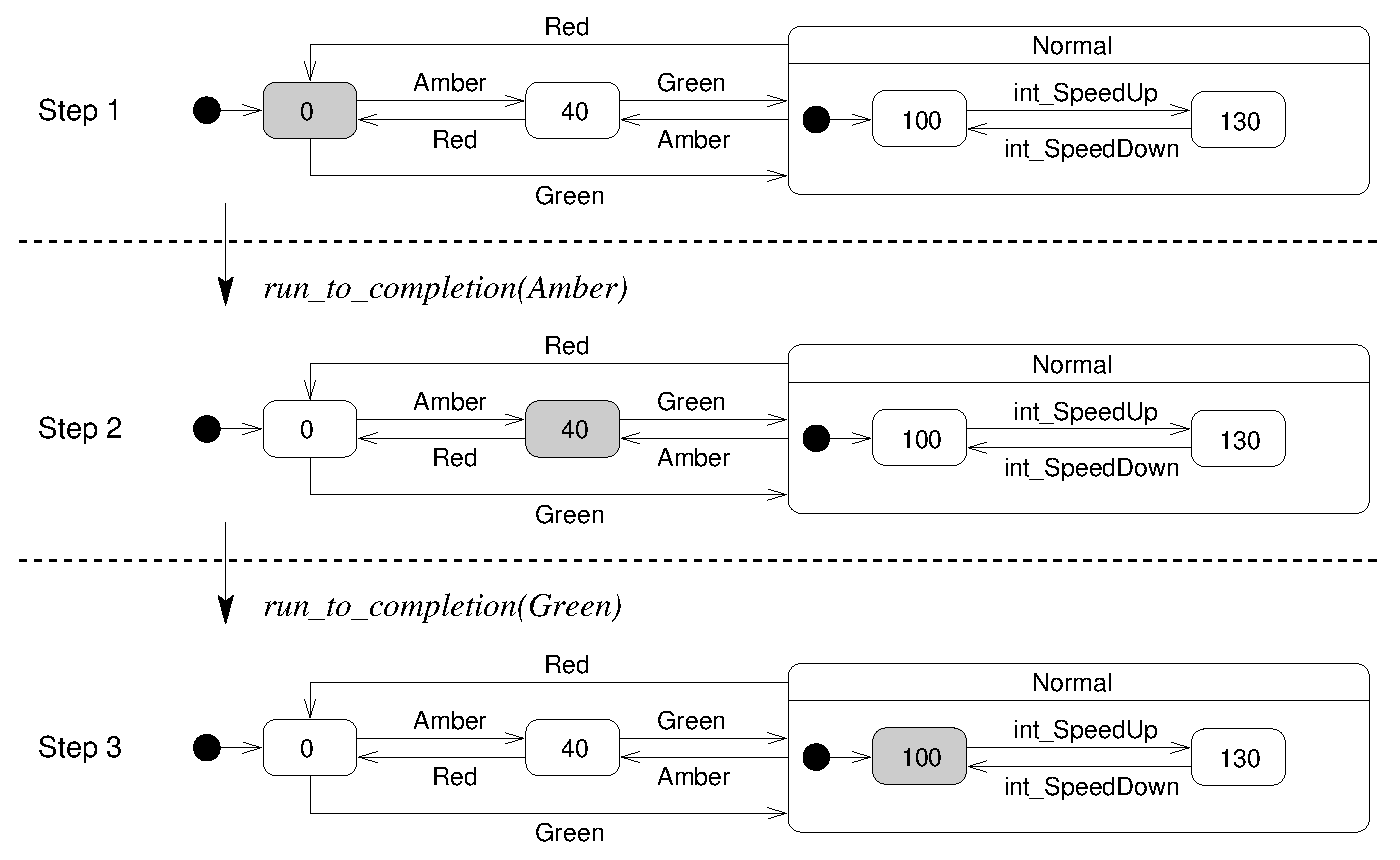
\epsfig{file=figures/train-exec.eps, width=11cm}
\caption{A train state machine execution}
\label{train-exec}
\end{center}
\end{figure}

The figure~\ref{train-exec} represents a state machine defining the
behavior of a non high-speed train and some steps of its
execution. Concretely, this train is not able to run at more than 130
km/h but is allowed to run at this speed on high-speed sections. The
states define the speeds of the train. For simplifying, the name of a
state is the train speed in km/h associated with this state. 0 and 40
are then speeds of 0 km/h and 40 km/h, that is the stop state and the
low speed state. When running at a normal speed, the train driver can
choose between two speeds, either 100 or 130 km/h. These two states
have been put into a composite one representing the normal
speeds. Transitions between states are associated with the signal
color lights: \textit{red}, \textit{green} and \textit{amber}. The
\textit{purple} color is not managed here, as the train cannot run at
more than 130 km/h, but it can run at 100 or 130 km/h on a high speed
section. There are two particular events: \texttt{int\_SpeedUp} and
\texttt{int\_Speed\-Down}. These events are internal actions of the
train, that is, correspond to direct train driver actions. For not
confusing them with the external events coming from the execution
environment, their names is prefixed by ``int\_''.

\subsubsection{Execution of the Train State Machine.}

The figure~\ref{train-exec} shows three steps of execution of the
state machine, through the \texttt{run\_to\_completion} operation
taking an event name as parameter. This operation processes an event
occurrence. The first step is the initial active configuration of the
state machine: Its initial state \texttt{0} is active (an active state
is graphically represented with a grey background). Then, for the second
step, the \texttt{Amber} event occurs and it makes changing the
current active state that is now the \texttt{40} one. Finally, the
third step is the result of the \texttt{Green} event occurrence which
leads to activate the \texttt{Normal} state and in consequence its
initial state, the state \texttt{100}.

Processing a state machine execution consists only in modifying the
\texttt{isActive} attribute value for the states and, for composite
states, in changing the referenced state of its potential history
state. As a conclusion, only the dynamical elements of the model are
modified during the execution.

\section{Characterization of Adaptable i-DSML}
\label{adaptable-iDSML}

We consider that an adaptable i-DSML is the logical extension of an
i-DSML. Indeed, adaptable models are executable models endowed with
adaptation capabilities. 


\subsection{The Design of an Adaptable i-DSML}

Figure~\ref{adapt-iDSML} depicts the design of an adaptable i-DSML. As
an adaptable i-DSML is an extension of an i-DSML, this figure extends
the figure~\ref{iDSML}. The added elements are:

\begin{enumerate}
	\item Meta-elements which express properties on the model and
          that should help its adaptation;
	\item Adaptation semantics, leveraging from the aforesaid
          properties, which express the adaptation problem and its
          solution.
\end{enumerate}

Item (1) makes reference to any structural elements and their
well-formedness rules that are added in the meta-model and whose role
is to facilitate the subsequent adaptations. This is called the
Adaptation Part. Item (2) denotes the adaptation semantics that is a
specialization of an execution semantics. Indeed, while execution
semantics prescribes a nominal behavior, the adaptation semantics
expresses also a behavior but for extra-ordinary or abnormal
situations requiring an adaptation. Again, an adaptation semantics can
be declined under the specification form for complementing the
meta-model definition~\cite{cariou-ciel12}, or under the operational
form. As a consequence, an adaptation engine implementing the
adaptation semantics is an extension of an execution engine: It
processes both the execution-related operational semantics and the
adaptation-related operational semantics.

Without going into details of how an adaptation semantics is managed
or processed by the engine, we can say that it will mainly be composed
of a set of fine-grained adaptation operations combined by a set of
rules. Some operations are dedicated to checking the consistency of
the model and others are actions concretely realizing the
adaptation. The rules are expressed under the form
``\texttt{if <check> then <action>}'' and any more complex or
recursive combination of the same kind.

The major point is that the adaptation semantics applies on elements
of all constituents of the adaptable i-DSML: All the structural parts
(static, dynamic and adaptation) and the behavioral ones (execution
semantics and adaptation semantics) are concerned. Concretely, at
runtime, the model's entire content can be changed including the
executed semantics. This brings reflexivity to the adaptable i-DSML
since enabling the adaptation of the adaptation (\textit{i.e.}
meta-adaptation).

\begin{figure}[htbp]
\begin{center}
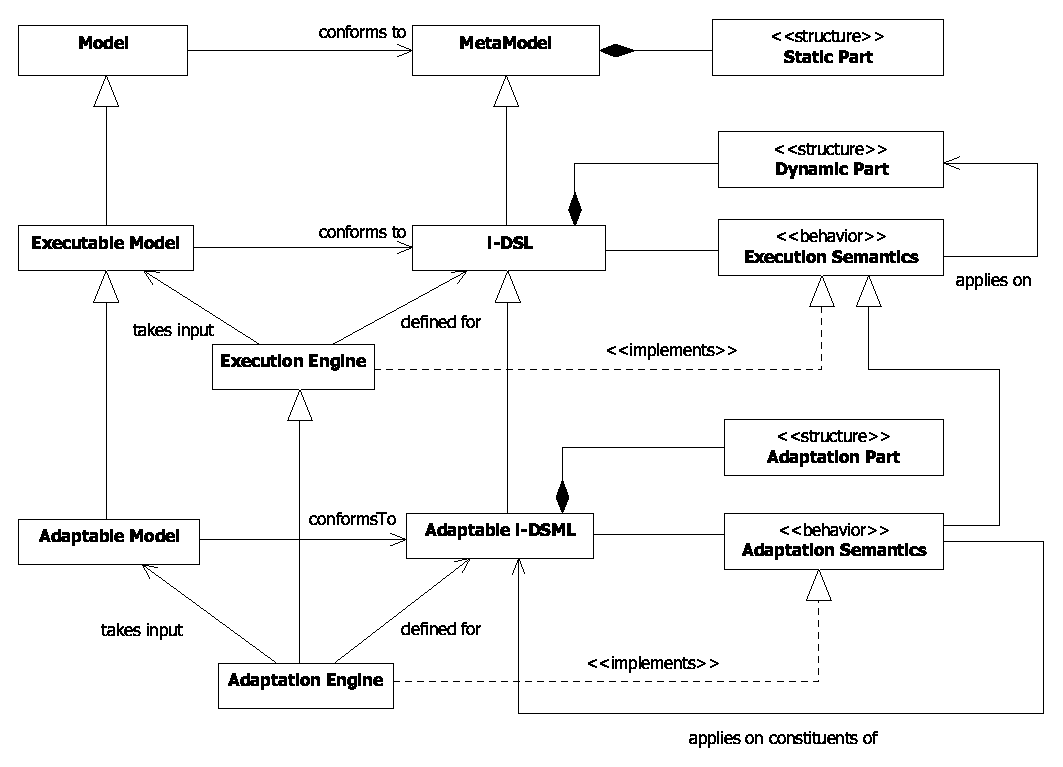
\epsfig{file=figures/adapt-iDSL, width=12.5cm}
\caption{Conceptual framework for adaptable i-DSML}
\label{adapt-iDSML}
\end{center}
\end{figure}


\subsubsection{Categories of Adaptation Actions.}

We identified two categories of adaptation actions:
Create/Update/Delete (CUD) and Substitution. CUD actions target
instances of any structural parts (static, dynamic, and adaptation).
Substitution is an action which targets the behavioral parts
(execution and adaptation semantics). We consider only substitution
for behavioral parts because it is not feasible to define a new
semantics from scratch (concretely, it will consist in writing lines
of code in the engine). Instead, having a set of existing semantics
(\textit{i.e.} already implemented) and choosing at runtime which of
them to process is straightforward. CUD and substitution can be
applied with the following purposes:

\begin{itemize}
\item CUD on the dynamic part: The current state of execution is
  altered (\textit{e.g.} force to go back/go forward, restart such as
  activating a given state for a state machine),
\item CUD on the static part: The structure of the model itself is
  changed (\textit{e.g.} modification of the modelized process such as
  adding a state or changing the initial state of a composite for a
  state machine),
\item CUD on the adaptation part: An adaptation-related element is
  changed (\textit{e.g.} the value of a QoS property is modified
  accordingly to a changing execution environment),
\item Substitution on the execution semantics: Switch from a given
  interpretation of the model to another one (\textit{e.g.} managing
  execution variants such as the Harel vs UML transition conflict
  semantics for state machines),
\item Substitution on the adaptation semantics: Switch from a given
  set of adaptation operations to other ones within the adaptation
  rules (\textit{e.g.} checking the consistency of the model with the
  execution environment in an exact or fail-soft mode).
\end{itemize}

\begin{table}
\caption{Adaptation and execution characteristics}
\label{table-resume}
\begin{center}
\begin{tabular}{|c|c|c|c|}
\hline
\multicolumn{2}{|c|}{\textbf{Elements of adaptable i-DSML}} & \textbf{Execution actions} & \textbf{Adaptation actions}\\
\hline
  \multirow{3}{*}{$<<$Structure$>>$} & Static Part & N/A & Create/Update/Delete \\
    & Dynamic Part & Create/Update/Delete & Create/Update/Delete \\
    & Adaptation Part & N/A& Create/Update/Delete \\ \hline
  
  \multirow{2}{*}{$<<$Behavior$>>$} & Execution Semantics & N/A & Substitution \\
    & Adaptation Semantics & N/A & Substitution \\ \hline
\end{tabular}
\end{center}
\end{table}

Table~\ref{table-resume} sums up these categories of adaptation
actions and contrasts with the actions processed by a simple model
execution. Indeed, in this case, only the dynamic part of the model is
modified whereas for model adaptation, all parts and semantics can be
changed.

\subsection{Adaptation Part for the State Machine Meta-Model}

The meta-model of state machines of the figure~\ref{mm-sm-adapt}
includes elements dedicated to the adaptation management. The first
one is the \texttt{elementKind} attribute available for the
\texttt{Event}, \texttt{Transition} and \texttt{State} elements
through the specialization of \texttt{AdaptableElement}. This
attribute allows the definition of ``kinds'' for events, transitions
and states of a state machine. A kind has for goal to precise that an
element is playing a particular role. Conceptually, a kind is
equivalent to a stereotype of UML profiles. In addition, through the
\texttt{properties} association, events, transitions and states can be
associated with properties. A property is basically composed of a name
and a value. For simplicity, only integer properties are considered
here, but of course, properties of any type could be added on the
meta-model (the definition of properties can of course be based on
reusing existing adaptation works, such as~\cite{fleurey09} which
defines a generic meta-model for specifying properties and associated
rules depending on their values). Properties can deal if required with
QoS parameters and values. Conceptually, a property is equivalent to a
tagged value of UML profiles.

As shown in the following, kinds and properties can be used for
managing the adaptation of a state machine execution thanks to the
additional information they offer. Kinds can be used to define
fail-soft mode of consistency against an execution
environment. Properties associated with events of the execution
environment enable the modification of the executed state machine for
managing unexpected events.

\subsection{Runtime Adaptation of the Train State Machine}

\begin{figure}[htbp]
\begin{center}
\epsfig{file=figures/train-adapt.eps, width=\textwidth}
\caption{Adaptation of the train state machine}
\label{train-adapt}
\end{center}
\end{figure}


The main adaptation rule consists in first checking if the behavior of
the system is consistent with the execution environment, that is
concretely here, if any signal is understandable and correctly
processed by the train state machine. Secondly, when the system is not
consistent with the environment, to perform an adaptation action such
as switching in a fail-soft checking mode or modifying the structure
of the model.

As explained in~\cite{cariou-ciel12,cariou-mrt12}, specific design
constraints can be applied for verifying the consistency of a model
against an execution environment. The problem is that it is necessary
to be able to distinguish an unexpected interaction -- requiring to
take an adaptation decision -- from an expected and already managed
one. For state machines, it is required to be able to determine if an
event is expected or not. Several solutions are possible, such as
parameterizing the execution engine with the list of expected events
and to verify for each event occurrence if it is in the
list. The solution applied here is self-contained in the model by
adding explicitly a transition starting from each state for each
expected event. Figure~\ref{train-adapt}, part (a), shows the
modification of the train state machine: For every expected
color events (\textit{red}, \textit{amber}, \textit{green} and
\textit{purple}), there is a transition starting from each state. When
a color event leads to remain in the same state, it is a
self-transition (leading to the historical state of a composite for
composite states). Now, excepting for internal events starting by
``int\_'', each event, corresponding to a color of signal crossed by
the train, triggers a transition. If no transition is associated with
an event according to the current active states, then this event is
unexpected and an adaptation action has to be performed.

Based on this new train state machine definition, as an illustration,
we describe here seven adaptation operations (two adaptation checking
and five adaptation actions including one modifying the adaptation
semantics) and two execution semantics variants for the state machine
meta-model.

\subsubsection{Adaptation Checking.}

The main verification is to determine if an event is expected or
not. This verification can be made in an exact mode or in a fail-soft
mode through the kinds of events. Let us consider the occurrence of the
\textit{purple} signal event. The train is not able to run at a high
speed level, so, when crossing such a \textit{purple} signal, the
train will run at a normal speed. For this reason, the train state
machine of figure~\ref{train-adapt} part (a) leads to the state
\texttt{Normal} for each occurrence of the \textit{purple} event.

The exact mode consists in verifying that there is a transition
associated with the exact event (through its name) and the fail-soft
mode that there is a transition for the kind of event and not
necessary for the exact event. Figure~\ref{train-adapt}, part (b),
shows a variant of the train state machine where kinds and properties
have be added onto states and events. There are three kinds of states
(the kinds are represented through the $<<..>>$ UML stereotype
notation): The \texttt{0} state is a stop state, the \texttt{40} one
is a low speed state and the composite state \texttt{Normal} is a
normal speed state. The events, depending of their associated target
state\footnote{We rely on a dedicated restriction on the state
  machines: All transitions associated with a given event are always
  leading to the same state. For instance for the train state machine,
  independently of the source state, the \textit{amber} event always
  leads to the state \texttt{40}.}, are also tagged with kinds:
\textit{red} is a stop event, \textit{amber} is a low speed event,
\textit{green} and \textit{purple} are normal speed events. One can
notice that transitions associated with the \textit{purple} color have
disappeared. Indeed, in a fail-soft mode, the \textit{purple} event
will be processed as the \textit{green} one because there come from
the same normal kind. The \textit{purple} color is for the train
considered as a \textit{green} one even if they do not have the same
role and meaning.

The verification mode can be changed at runtime: A checking adaptation
operation can be substituted by another one (changing in that way the
adaptation semantics). If the model of the figure~\ref{train-adapt},
part (b), is executed and if the train is running on normal speed
sections, then the verification mode can be the exact one because the
\textit{red}, \textit{amber} and \textit{green} signals that can be
crossed are directly and exactly processed for each state of the state
machine. However, if the train is now running on a high-speed section,
it can cross a \textit{purple} signal that is not directly processed
in the exact mode. An adaptation action can be to switch into a
fail-soft verification mode and to recheck the validity of the
\textit{purple} signal. In this mode, as explained, this signal will
be considered as a \textit{green} one and will be processed.

From an implementation point of view, our Kermeta execution engine has
been extended for managing the adaptation. Mainly, a pre-condition has
been added for the \texttt{run\_to\_completion} operation that
processes each event occurrence. This pre-condition performs the chosen
adaptation checking and, if not respected, an adaptation action is
executed.

\subsubsection{Adaptation Actions.}

In addition to substituting an adaptation checking operation by
another one, several adaptation actions can be taken in case of
unexpected events, that is, in case of a changing execution
environment. A very basic action is to stop the execution of the state
machine if there is no way to decide how to handle the event. A more
relevant adaptation action is to load a new state machine (a reference
one as defined in~\cite{cariou-mrt12}) that is able to manage the new
execution environment if such a state machine is available.

If the unexpected event is associated with properties, they can be
used to determine if this event can target an existing state of the
state machine or, if not, to add the associated state and transitions
on the state machine. Figure~\ref{train-adapt}, part (b), defines a
speed property for each event and state. Properties are represented
similarly to tagged values of UML profiles (as the
\texttt{\{speed=XXX\}} ones). For instance, the \textit{amber} event
and the state \texttt{40} are both associated with a speed property of
the value 40, that is, 40 km/h. Let us suppose that, if this train
state machine is executed, a white signal, of a \texttt{reduced} kind and a
speed property of 70 km/h, is crossed. In both exact and fail-soft
verification modes, this white event is an unexpected one. As no state
has a speed property with a value of 70, a new state called
\texttt{70} is created with the same kind and speed property as the
white event. All required transitions, starting from or leading to
this new state, have also to be added: Each existing state must be the
source of a transition associated with the white event and leading to
this new state and for each color event (\textit{red}, \textit{amber} and
\textit{green}) there must be a transition starting from this new
state and leading to the required state. The figure~\ref{train-adapt},
part (c), shows the resulted runtime modification for managing the
white signal. An important point to notice about this model
modification is that it is based on the comparison of the properties
without requiring to know what they are and what they are
representing. The adaptation engine simply compares two sets of
properties through their names and values.

A last adaptation action could be to force the activation of the state
that is from a stop kind (the state \texttt{0} for the train state
machine) in case of an unexpected event (this action is different from
stopping the execution of the state machine as described above because
here the state machine is still being executed). The idea is that the
train stops if it does not understand a signal.

\subsubsection{Execution Semantics Variants.}

For state machines, a transition conflict appears when a transition is
starting from a composite state and that there is also a transition
associated with the same event starting from an internal state of this
composite. The way to choose which transition to fire when this event
occurs is a semantics variation point. According to the UML
semantics\footnote{\texttt{http://www.omg.org/spec/UML/2.2/}}, it is
the most internal one that is fired while the original Harel
statecharts semantics~\cite{harel87} leads to fire the external one
starting from the composite.

When loading a state machine model, including at runtime when changing
the current state machine by another one suited for a new context of
execution, it is required to know with which execution semantics it
was designed. We can imagine a property associated with the state
machine and precising which kind of transition processing variant
must be used. Then, the execution engine embeds the operational code
for each semantics and the right one is processed depending of this
property value. In other words, when changing the executed model as an
adaptation action, the current operational semantics can be
substituted by another one if needed.

\section{Related Work}

As written, several papers such
as~\cite{breton01,cariou-ecmfa11,clarke-book-iDSML13,combemale-jos09,combemale-apsec12,engels00,lehmann10,pons00}
have already studied model
execution. Section~\ref{iDSML-charaterization} summarizes the
consensual characterization of model execution based on these works.

Concerning the adaptation of model execution, as far as we know, there
are no other works except ours which have studied this
subject. \cite{cariou-ciel12,cariou-mrt12} have been used as a base
for defining the direct model execution characterization exposed in
this paper. The MOCAS platform~\cite{BHB09} defines a UML agent state
machine observing an executed business UML state machine and requiring
changes on its current state or structural content. The adaptation is
then made following common models@run.time adaptation techniques
(case (c) of figure~\ref{img_loops}). The problem is that the
adaptation and the execution operations are strongly mixed-up in the
implementation platform. This leads to the absence of separation of
the adaptation logic from execution. Moreover, the platform does not
enable to replace at runtime the adaptation or execution semantics as
we propose.

\cite{lehmann10} offers a characterization of models at
runtime and related adaptation in the same spirit of this paper. But
there are two main differences with our characterization of direct
adaptation of model execution: (a) It always considers that the model,
even when executable, is causally connected with a running system
whilst for us the executed model is by essence the system and (b) it
does not go as far as us about the elements that can be modified by
the adaptation: It does not consider that the execution semantics or
the adaptation semantics can be changed.

\section{Conclusion}

In this paper we propose a conceptual characterization of the direct
adaptation of model execution, through the concept of adaptable
i-DSML. Albeit model execution and adaptation are closely related (as
an adaptation semantics is a specialized execution semantics), there
are two sharp demarcation lines. The first one, from a general point
of view, is about the intention embodied in the semantics. Indeed, an
execution semantics deals with a nominal behavior whereas an
adaptation one concerns extra-ordinary or abnormal situations. The
second one, from a technical point of view, is that model execution
only modifies the dynamic elements of the model whereas model
adaptation can modify each part of the model and the execution and
adaptation semantics.

The presented execution and adaptation engine is a first prototype
showing the interest of studying the adaptation of an executed model.
We need to develop more realistic and complex case studies and to
consider the adaptation of other kinds of adaptable i-DSML. Notably,
we plan to extend our existing tools dedicated to execute full
standard UML state machines:
SimUML\footnote{\texttt{http://sourceforge.net/projects/simuml/}} is a
simulation tool at the design level and
PauWare\footnote{\texttt{http://www.pauware.com/}} a Java library
implementing and executing UML state machines for any Java platform,
including Android devices. The goal is to define and implement
adaptation operations and semantics for UML state machines. We plan
also to enhance our MOCAS platform for making it clearly separating
the adaptation from the execution. These platforms and complex case
studies will allow us to study the limits of directly adapting a model
execution versus applying common models@run.time techniques on it. One
of our perspective is to determine when one approach is more suited
than the other one. Finally, just as an action language is provided
for expressing the execution semantics, a mid-term perspective is to
provide a full-fledged adaptation language. This DSML will support the
adaptation loop by offering language constructs for both checking and
actions. Concretely, it will enable to define separately the execution
logic and the adaptation one, and then to express how the adaptation
checking and actions are orchestrated and weaved with the execution
operations.


\bibliographystyle{abbrv}
\bibliography{biblio}

\end{document}
